%!TEX program = xelatex
\documentclass[cn,hazy,blue,14pt,screen]{elegantnote}
\title{Exia:平衡机器算法全生命周期管理工具}

\author{施华}
\institute{Exia Algorithm Manager}

\version{beta-0.1}
\date{\zhtoday}

\usepackage{array}

\begin{document}

\maketitle

\centerline{
  
\includegraphics[width=0.2\textwidth]{logo-ae.png}
}



\section{Exia Algorithm Manager介绍}

Exia Algorithm Manager主要针对算法开发中开发标准不统一,生产环境部署复杂,算法管理混乱三大痛点来设计构建,是一个纯Python语言工具包,采用OOP编程范式,Pythonic代码风格。

Exia Algorithm Manager有下面几个特性:

\begin{itemize}
  \item 运行时动态添加插件
  \item 插件开发度高,可自由组合
  \item 提供功能完善的基础套餐(数据获取,模型管理,模型监控,算法记录,服务管理)
\end{itemize}

以下主要是主体框架和基础套餐的设计说明



\subsection{主体框架}

Exia Algorithm Manager主要实现了动态添加插件,自由配置插件的功能。主要涉及的技术有:

\begin{enumerate}[label=\arabic*).]
	\item \textit{对象池技术}\\
	仿造游戏编程中的对象池技术,将功能组件对象化后放入对象池,这就实现了动态添加插件功能。
	\item \textit{DAG技术}\\
	引入DAG数据结构用于存储组件实例化构建逻辑,借助Python动态语言特性,实现自由配置插件和自由配置组件的功能。DAG模块中包含了自定义的DAG数据结构类和拓扑排序算法
	\item \textit{描述符协议}\\
	主要用于对象池中对象实例的属性管理和方法绑定,使得扩展更灵活。
	\item \textit{上下文管理协议}\\
	主要用于对象池资源的管理,防止内存泄漏
	\item \textit{单例模式}\\
	主要用于池化对象,使得对象池中的对象都是一个单例。
	\item \textit{命令模式}\\
	主要用于实现依赖倒置原则,解耦上下层。
	\item \textit{eval技术}\\
	主要用于实时运行字符串
	\item \textit{工厂模式}\\
	主要采用静态方法和类方法实现,提供灵活扩展选项。
\end{enumerate}

\centerline{
	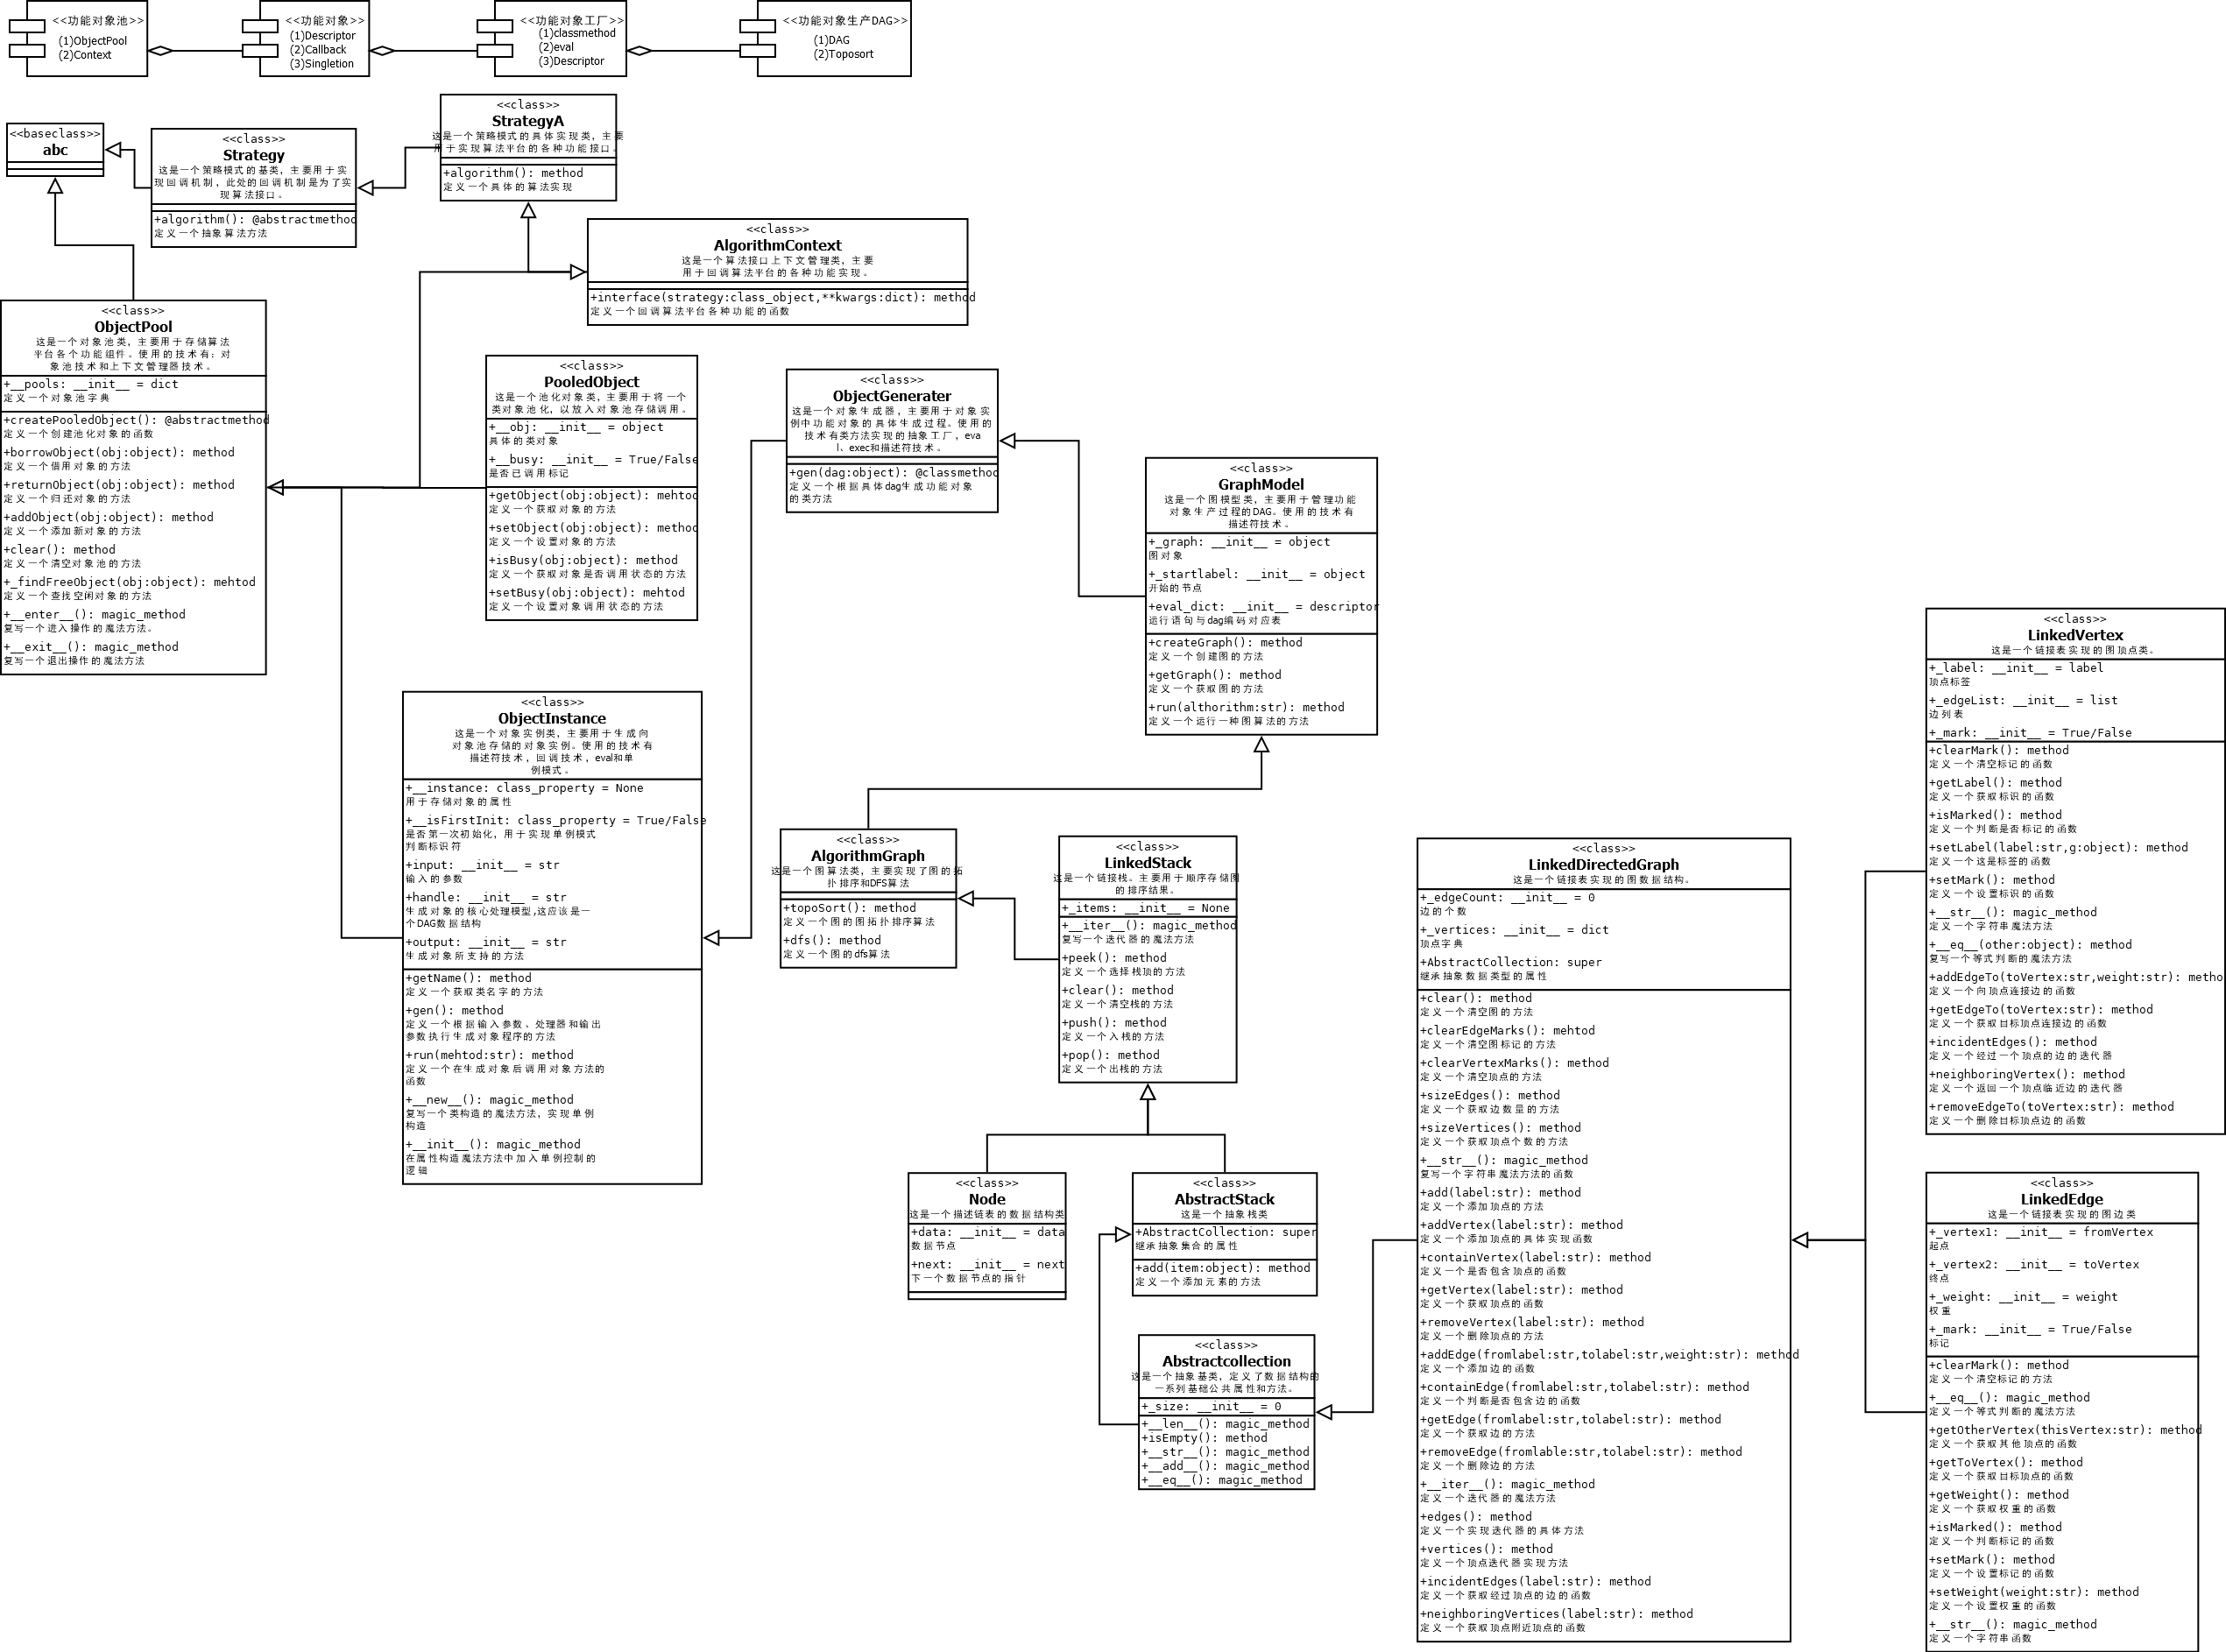
\includegraphics[width=0.8\textwidth]{AlgorithmManager.png}
}



\subsection{基础套餐}

基础套餐主要包括数据获取、模型管理、模型监控、算法记录、服务管理五大功能模块



\subsubsection{DataAPI}

DataAPI作为算法的数据接入层,提供算法和数据间的中间层,实现算法和数据的隔离。主要涉及的技术有:
\begin{enumerate}[label=\arabic*).]
	\item \textit{构建模式}\\
	主要用于各类数据库Python接口类的组建,注重过程。
	\item \textit{组合模式}\\
	主要用于辅助构建各类数据库操作类的构建。
\end{enumerate}

\centerline{
	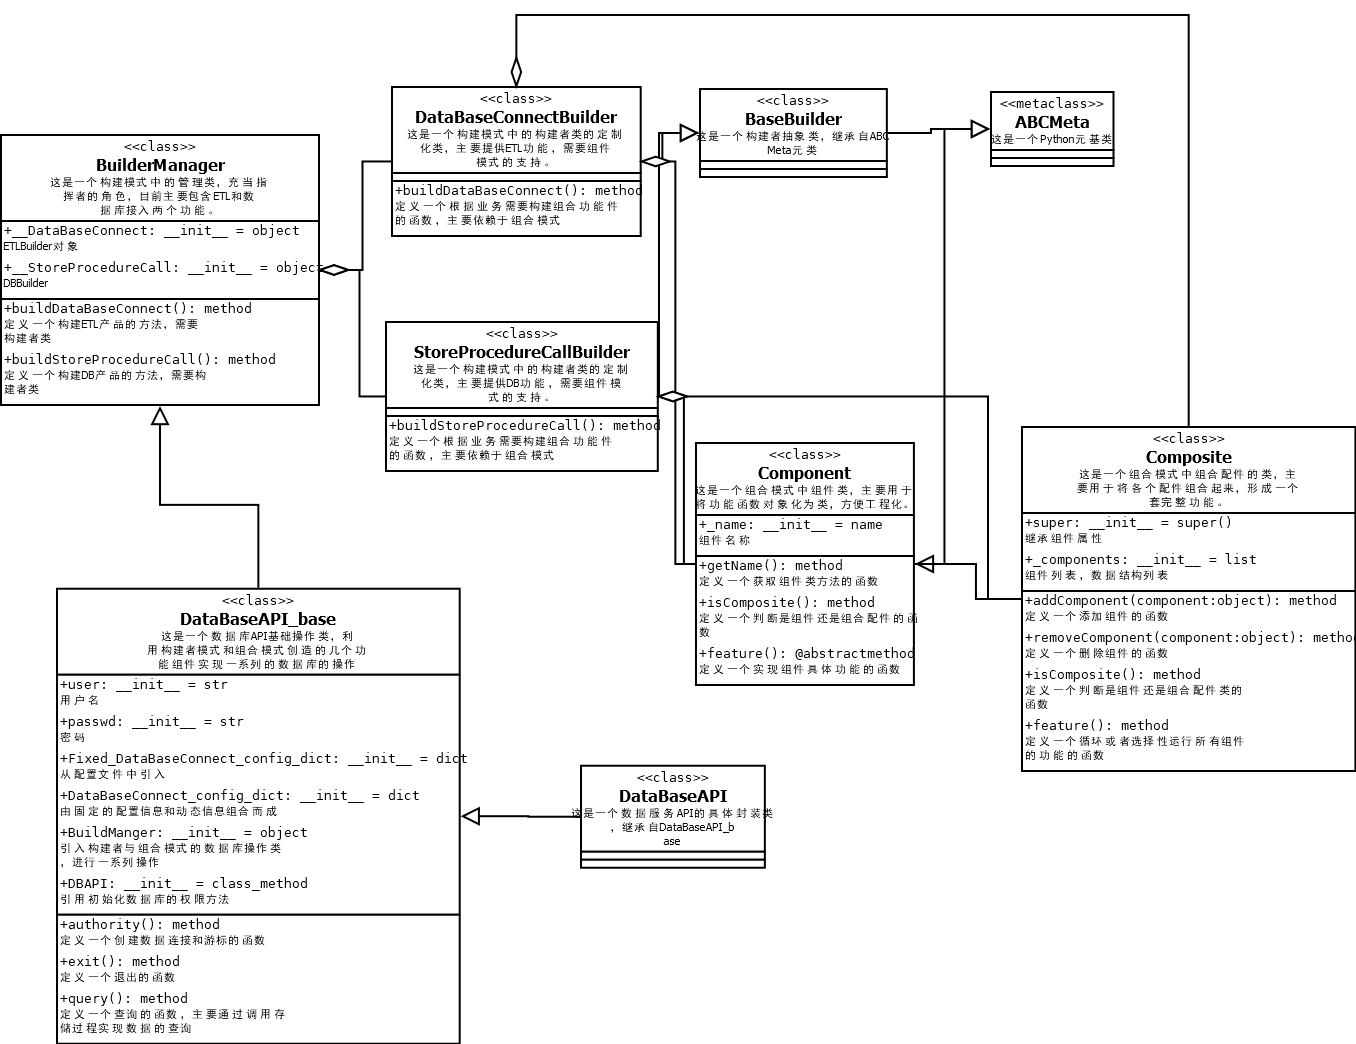
\includegraphics[width=0.8\textwidth]{DataAPI.png}
}




\subsubsection{ModelLibrary}

ModelLibrary作为算法管理层组件,提供模型管理功能,实现模型训练和推理解耦,提高算法运行效率。主要涉及的技术有:
\begin{enumerate}[label=\arabic*).]
	\item \textit{命令模式}\\
	主要用于实现依赖倒置原则,解耦上下层。
	\item \textit{MinIO}\\
	主要用于模型的对象存储,方便快捷。
	\item \textit{MinIO}\\
	主要用于模型的对象存储,灵活配置。
	\item \textit{MongoDB}\\
	主要用于模型信息的存储,方便模型回退和模型选择。	
\end{enumerate}

\centerline{
	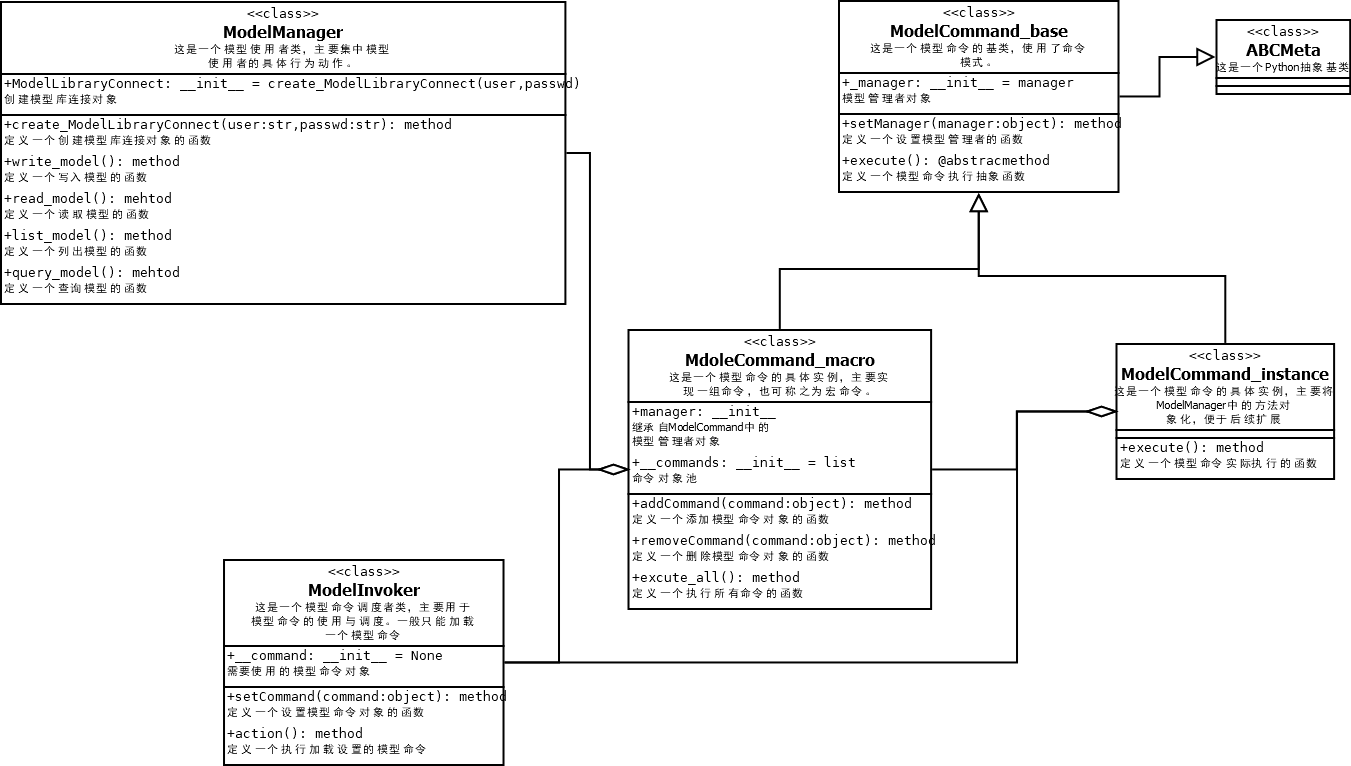
\includegraphics[width=0.8\textwidth]{ModelLibrary.png}
}



\subsubsection{ModelMonitoring}

ModelMonitoring作为算法管理层组件,提供模型监控功能,实现模型更新,形成算法闭环。主要涉及的技术有:
\begin{enumerate}[label=\arabic*).]
	\item \textit{观察者模式}\\
	主要用于监控模型指标。
	\item \textit{命令模式}\\
	主要用于实现依赖倒置原则,解耦上下层	
\end{enumerate}

\centerline{
	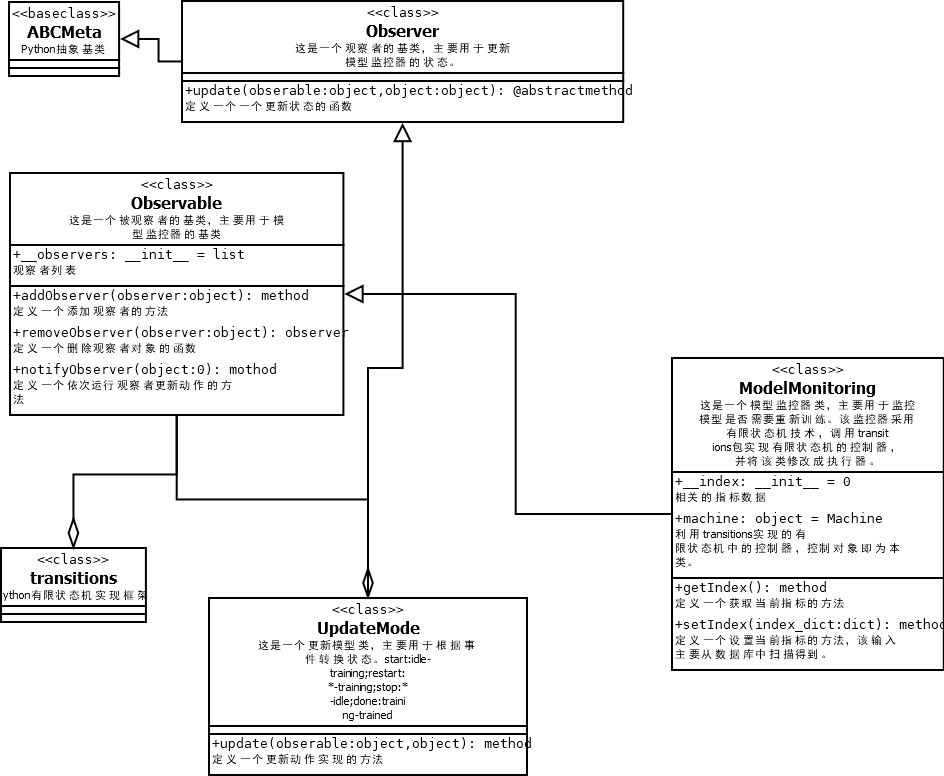
\includegraphics[width=0.8\textwidth]{ModelMonitoring.png}
}



\subsubsection{ServerManager}

ServerManager作为算法服务层组件,提供算法服务构建,算法服务管理,参数管理,远程操作功能。主要涉及的技术有:
\begin{enumerate}[label=\arabic*).]
	\item \textit{工厂模式}\\
	主要用于生成各种功能命令对象。
	\item \textit{有限状态机}\\
	主要用于模型状态监控,更新模型。	
	\item \textit{Consul}\\
	主要用于参数管理和服务管理。
	\item \textit{SSH}\\
	主要用于远端操作。
	\item \textit{AirFlow}\\
	主要用于算法工作流组合和调度。
\end{enumerate}

\centerline{
	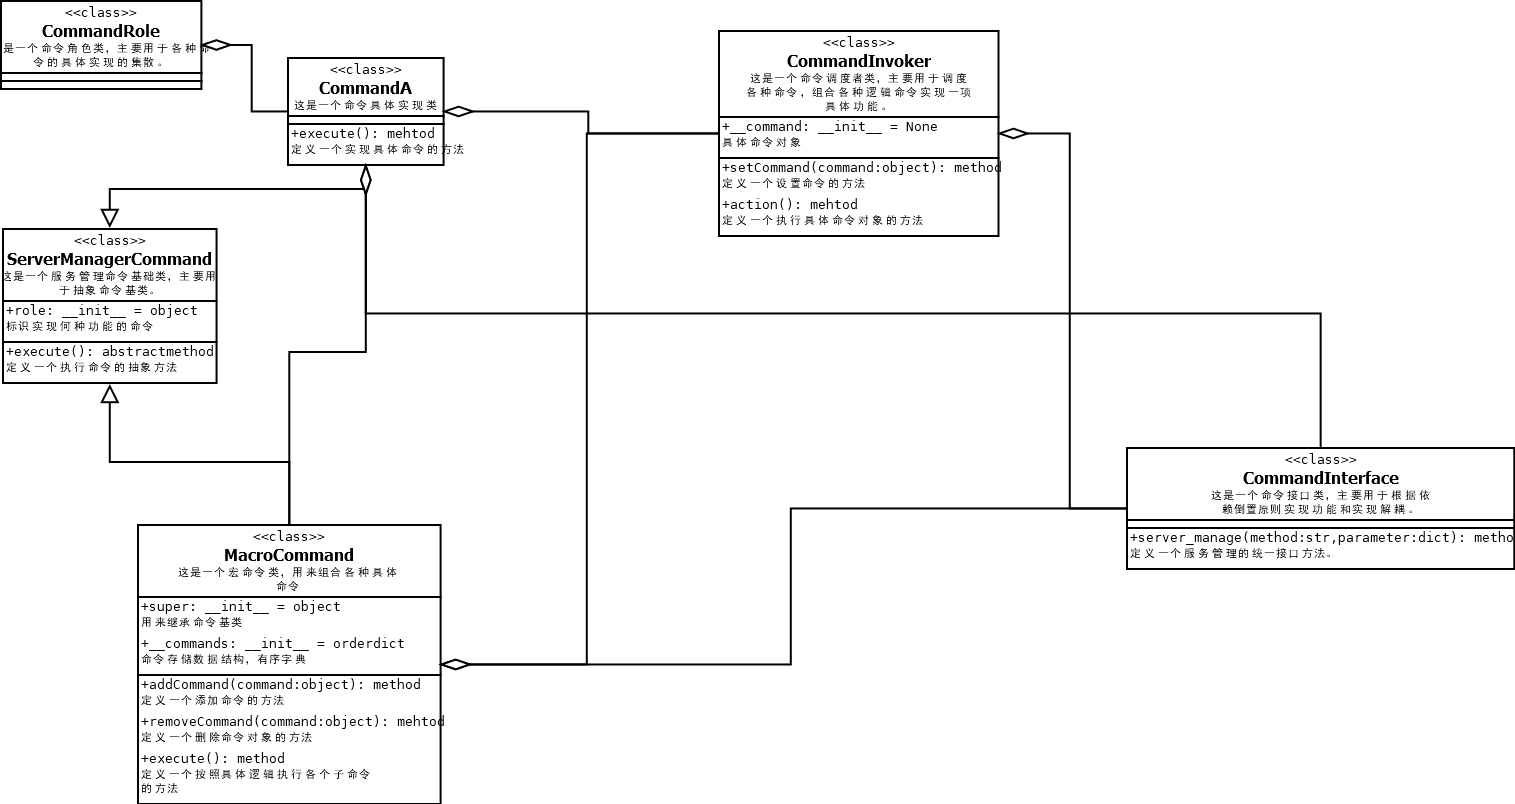
\includegraphics[width=0.8\textwidth]{ServerManager.png}
}



\subsubsection{LogDecoratorEK}

LogDecoratorEK作为算法管理层组件,提供算法日志记录功能。主要涉及的技术有:

\begin{enumerate}[label=\arabic*).]
	\item \textit{装饰器模式}\\
	主要提供算法记录功能,对代码百分百无侵入。
	\item \textit{ElasticSearch}\\
	主要用于算法记录后端。	
	\item \textit{Kibana}\\
	主要用于算法记录可视化。\\
\end{enumerate}

\centerline{
	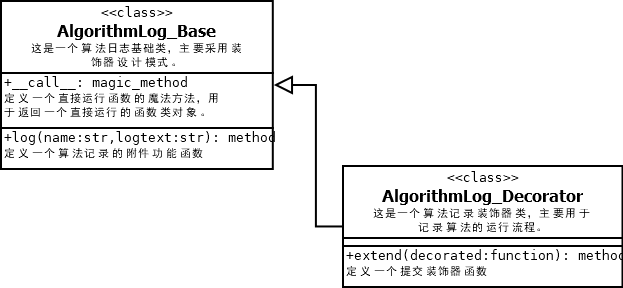
\includegraphics[width=0.8\textwidth]{LogDecoratorEK.png}
}



\subsection{使用示例}

Exia的动态插件功能可运行时直接引入组件模块,无须重新编译,组件模块配置灵活,具有较强的扩展性。具体使用步骤如下:

\begin{enumerate}[label=\arabic*).]
	\item \textit{实例化策略管理器和对象池:}\\
	对象池创建提供基础套餐和空对象池两种方案,基础方案需要初始化数据库配置参数。
	\item \textit{在With环境中使用对象池,对象池支持的操作有}\\
	从对象池中借用对象\\
	查看对象支持的主要使用方法\\
	根据主要使用方法调用具体方法(根据具体包的设计不同而定)\\
	返回对象\\
	清空对象池(如果不适用With环境或需要清空操作,可使用此方法)\\
	获取对象池
\end{enumerate}

代码示例:

\begin{lstlisting}
	### 引入代码包
	from AlgorithmManager.StrategyInterface.Strategy import * 
	
	
	
	### 实例化策略管理器和对象池
	StrategyContext = StrategyContext()
	ObjectPool = ObjectPool('test_pool')
	
	
	
	### 使用基础套餐
	ObjectPool = StrategyContext.interface(strategy = StrategyObjectPoolBase(ObjectPool = ObjectPool),
	DataAPI_user = 'root',
	DataAPI_passwd = '123456',
	DataAPI_host = '10.2.12.248',
	DataAPI_port = 3306,
	DataAPI_db = 'test',
	DataAPI_charset = 'utf8')
	
	
	
	### 在With环境中使用对象池
	with ObjectPool as ObjectPool:
	
	
	
	### 从对象池中借用对象
	ShowInfo = ObjectPool.borrowObject('ShowInfo')
	ModelMonitoring = ObjectPool.borrowObject('ModelMonitoring') 
	DataAPI = ObjectPool.borrowObject('DataAPI')
	LogDecoratorEK = ObjectPool.borrowObject('LogDecoratorEK')
	ModelLibrary = ObjectPool.borrowObject('ModelLibrary')
	ServerManager = ObjectPool.borrowObject('ServerManager')
	
	
	
	### 使用对象
	ShowInfo.ShowInfo(ObjectPool,'ModelMonitoring')
	ShowInfo.ShowInfo(ObjectPool,'DataAPI')
	ShowInfo.ShowInfo(ObjectPool,'LogDecoratorEK')
	ShowInfo.ShowInfo(ObjectPool,'ModelLibrary')
	ShowInfo.ShowInfo(ObjectPool,'ServerManager')
	
	
	## ModelMonitoring
	ModelMonitoring.setIndex(0.1)
	print(ModelMonitoring.state)
	
	
	## DataAPI
	
	# 调取存储过程
	weight = 110
	age = 29
	InputParameters_dict = {
		'args' : (weight,age),
		'procname' : 'getdata'
	}
	data = DataAPI.exec_stored_procedure(InputParameters_dict = InputParameters_dict)
	DataAPI.exit()
	print(DataAPI.DBAPI)
	print(data)
	
	
	## LogDecoratorEK
	
	# 手动打日志
	@LogDecoratorEK.extend
	def run_model(a,b):
	c = a + b
	print(">>>>>>",c)
	return c
	c = run_model(1,2)
	run_model.log(name='log_level_Test',logtext='Add log with consul!PKG First!',host = '10.2.12.248',port = 8500)
	
	
	## ModelLibrary
	def hahahe(name):
	print('Ha ha,{}'.format(name))
	def hello_world(name):
	print('Hello world,{}'.format(name))
	user = 'admin'
	passwd = '123456'
	db = 'test'
	collection_name = 'capped'
	mongodb_config_dict = {'host' : '10.2.12.248','port' : 27017}
	mode = 'trained_model_object_store'
	model_name = 'test_model'
	model_type = 'pkl'
	connect_info = '10.2.12.248:9000'
	access_key = 'minioadmin'
	secret_key = 'minioadmin'
	secure = False
	object_file = 'test_model.pkl'
	bucket = 'testdata'
	
	# 写入Pthon对象
	write_result = ModelLibrary.WriteModel(user = user,
	passwd = passwd,
	db = db,
	collection_name = collection_name,
	mongodb_config_dict = mongodb_config_dict,
	mode = 'direct_operation',
	model_name = 'hahahe',
	model_instance = hahahe)
	print(write_result)
	
	# 写入模型对象
	write_result = ModelLibrary.WriteModel(user = user,
	passwd = passwd,
	db =db,
	collection_name = collection_name,
	mongodb_config_dict = mongodb_config_dict,
	mode = mode,
	model_name = model_name,
	model_type = model_type,
	connect_info = connect_info,
	access_key = access_key,
	secret_key = secret_key,
	secure = secure,
	object_file = object_file,
	bucket = bucket)
	print(write_result)
	
	# 读取Python对象
	read_result = ModelLibrary.ReadModel(user = user,
	passwd = passwd,
	db =db,
	collection_name = collection_name,
	mongodb_config_dict = mongodb_config_dict,
	mode = 'direct_operation',
	model_name = 'hahahe')
	print(read_result)
	read_result('shihua')
	
	# 读取模型对象
	read_result = ModelLibrary.ReadModel(user = user,
	passwd = passwd,
	db =db,
	collection_name = collection_name,
	mongodb_config_dict = mongodb_config_dict,
	mode = mode,
	model_name = model_name,
	model_type = model_type,
	connect_info = connect_info,
	access_key = access_key,
	secret_key = secret_key,
	secure = secure,
	object_file = object_file,
	bucket = bucket)
	print(read_result)
	
	
	## ServerManager
	log_config_dict = {
		'LOG_ENABLED' : True,
		'LOG_TO_CONSOLE' : True,
		'LOG_TO_FILE' : True,
		'LOG_TO_ES' : True,
		'LOG_PATH' : './runtime.log',
		'LOG_LEVEL' : 'INFO',
		'LOG_FORMAT' : '%(levelname)s - %(asctime)s - process: %(process)d - %(filename)s - %(name)s - %(lineno)d - %(module)s - %(message)s',
		'ELASTIC_SEARCH_HOST' : '10.2.12.248',
		'ELASTIC_SEARCH_PORT' : 9200,
		'ELASTIC_SEARCH_INDEX' : 'runtime',
		'APP_ENVIRONMENT' : 'dev'
	}	
	Fixed_DataBaseConnect_config_dict = {
		'host' : '10.2.12.248',
		'port' : 3306,
		'db' : 'test',
		'charset' : 'utf8',
	}
	
	# 写入参数
	tmp_value = ServerManager.InputParameter(host = "10.2.12.248",
	port = 8500,
	key = 'log_config_dict',
	value = str(log_config_dict))                                   
	print("=============>",tmp_value)       
	
	# 读取参数                                             
	tmp_value = ServerManager.GetParameter(host = "10.2.12.248",
	port = 8500,
	key = 'log_config_dict')
	print("==========>",tmp_value)          
	
	# 根据模板生成文件                                           
	tmp_value = ServerManager.GenerateJinjia2(searchpath=r"D:\AEwork\algorithm_platform\Demo\airflow_dag",
	template_name = 'test_dag',
	parameter_dict = {'tmp_func':'TestTrain'},
	output_filepath = 'tmp_testtest.proto')
	print("===============>",tmp_value)
	
	# 写入对象
	tmp_value = ServerManager.PutObject(connect_info = '10.2.12.248:9000',
	access_key = 'minioadmin',
	secret_key = 'minioadmin',
	secure = False,
	object_file = 'train_data.csv',
	bucket = 'testdata')
	print("===============>",tmp_value)
	
	# 读取对象
	tmp_value = ServerManager.GetObject(connect_info = '10.2.12.248:9000',
	access_key = 'minioadmin',
	secret_key = 'minioadmin',
	secure = False,
	object_file = 'HS300.csv',
	bucket = 'testdata')
	print("===============>",tmp_value)
	
	# 删除对象
	tmp_value = ServerManager.OSRemove(filepath = 'tmp_testtest.proto')
	print("===============>",tmp_value)
	
	# 远端操作
	SSH_host_dict = {
		'host' : '10.2.12.248',
		'port' : 22,
		'username' : 'shihua',
		'pwd' : 'ATTACK7121553rb1'
	}
	command = 'service mysql status'
	tmp_value = ServerManager.SSHRunCMD(SSH_host_dict = SSH_host_dict,
	command = command)
	print("===============>",tmp_value)
	
	
	
	### 返回对象
	ObjectPool.returnObject('ModelMonitoring')
	
	
	
	### 清空对象池
	# ObjectPool.clear()
	
	
	
	### 获取对象池
	ObjectPool_test = ObjectPool.getObjectPool()
	print(ObjectPool_test)
	print("=========================================================================================")
	ObjectPool_test = ObjectPool.getObjectPool()
	print(ObjectPool_test)
\end{lstlisting}



\end{document}
